%-------------------------------------------------------------------------------------------------------------------------------------------
%	PACKAGES AND OTHER DOCUMENT CONFIGURATIONS
%-------------------------------------------------------------------------------------------------------------------------------------------

\documentclass[a4paper,11pt]{article} % Font and paper size

%----------------------------------------------------------------------------------------
%	PACKAGES AND OTHER DOCUMENT CONFIGURATIONS
%----------------------------------------------------------------------------------------

\usepackage[utf8]{inputenc} % Required for inputting international characters
\usepackage[T1]{fontenc} % Output font encoding for international characters
\usepackage[italian]{babel} % Italian dictionary


\usepackage[table]{xcolor} % Required for custom colors
\usepackage{gensymb}
\usepackage{amsmath}
\usepackage{bm}
\usepackage{tikz}
\usepackage{hhline}
\usepackage{listings}
\usepackage{enumitem}

%\usepackage[margin=2cm, includefoot]{geometry} % Modify margins
\usepackage{fancyhdr}
\usepackage{rotating}
\usepackage[hidelinks]{hyperref} % Hyperlinks

\usepackage[none]{hyphenat}% Non spezza le parole nelle tabelle
\usepackage{array}

\usepackage{graphicx} % Required for figures
\usepackage{float}
\usepackage{wrapfig}
\usepackage{caption}
\usepackage{subcaption}

%pagestyle
\pagestyle{fancy}
\fancyhead{}
\fancyfoot{}
\fancyfoot[R]{\thepage}
\renewcommand{\headrulewidth}{0pt}



\usepackage{xfrac}
\usepackage{amssymb}

\usepackage{multicol}
\usepackage{multirow}

\usepackage[toc, page]{appendix}
\usepackage{booktabs}
\usepackage{siunitx}


%----------------------------------------------------------------------------------------
%	NEW COMMANDS
%----------------------------------------------------------------------------------------

\newcommand{\restr}[2]{{% we make the whole thing an ordinary symbol
\left.\kern-\nulldelimiterspace % automatically resize the bar with \right
#1 % the function

\right|_{#2} % this is the delimiter
}}

\newcommand{\tnhl}{\tabularnewline\hline}
\newcommand{\tn}{\tabularnewline}
\newcolumntype{x}[1]{%
	>{\centering\hspace{0pt}}p{#1}}%


 % Include the file specifying document layout and packages


%-------------------------------------------------------------------------------------------------------------------------------------------
%	GENERAL INFORMATION 
%-------------------------------------------------------------------------------------------------------------------------------------------

\newcommand{\labcourse}{Laboratorio di Fisica}
\newcommand{\teacher}{Docenti: Prof. A. Garfagnini - Prof. M. Lunardon}
\newcommand{\laurea}{Corso di Laurea in Fisica}
\newcommand{\channel}{Canale 1 A-L}
\newcommand{\academicyear}{Anno Accademico 2020/2021}
\newcommand{\labexp}{Esperienza di Laboratorio}
\newcommand{\exptitle}{Catena Elettronica}
\newcommand{\turno}{Turno T2}
\newcommand{\name}{Nicolò Lai}
\newcommand{\matricola}{1193976}
\newcommand{\mail}{nicolo.lai@studenti.unipd.it}
\newcommand{\consegna}{Data Esperienza}
\newcommand{\data}{23/11/2020 \\ 25/11/2020 \\ 26/11/2020}


%-------------------------------------------------------------------------------------------------------------------------------------------
%	DOCUMENT 
%-------------------------------------------------------------------------------------------------------------------------------------------

\begin{document}

%-------------------------------------------------------------------------------------------------------------------------------------------
%	REFERNCE CUSTOMIZATION
%-------------------------------------------------------------------------------------------------------------------------------------------

\def\sectionautorefname{Sezione} 
\def\subsectionautorefname{Sezione} 
\def\subsubsectionautorefname{Sezione}

%-------------------------------------------------------------------------------------------------------------------------------------------
%	TITLE PAGE
%-------------------------------------------------------------------------------------------------------------------------------------------

\begin{titlepage}
	\begin{center}
		\Huge{\bfseries \labcourse}\\
			
		\LARGE \teacher \\
		\Large \laurea\\
		\Large \channel\\
		\Large \academicyear\\
		[1cm] 
		\line(1,0){400}\\
		[3.5cm]
			
		\textsc{\huge{\bfseries \labexp}}\\
		\huge{\exptitle}\\
		[2mm] \line(1,0){300}\\
		[9cm]
	\end{center}
	
	
	\begin{flushleft}
		\textsc{\Large \turno}\\
		[0.5cm] \textsc{\large {\bfseries \name}} \\ 
		\indent\large \matricola \\ 
		\indent\large \mail \\
	\end{flushleft}
		
					
	\begin{flushright}
			\textsc{\Large\consegna}\\
			\textsc{\large \data}					
	\end{flushright}
			
\end{titlepage}
\cleardoublepage


%-------------------------------------------------------------------------------------------------------------------------------------------
%	OBIETTIVO
%-------------------------------------------------------------------------------------------------------------------------------------------

\section{Obiettivo}

Assemblare i moduli principali costituenti una catena elettronica (\textit{preamplificatore}, \textit{shaper},
\textit{amplificatore}). Studiarne il segnale in uscita e la risposta in frequenza per ciascuno di essi.

%-------------------------------------------------------------------------------------------------------------------------------------------
%	APPARATO SPERIMENTALE
%-------------------------------------------------------------------------------------------------------------------------------------------

\section{Strumentazione e Componenti}\label{s:strumenti}

Nel corso dell'esperienza vengono utilizzati:
\begin{itemize}[itemsep=-0.5ex]
	\item Multimetro digitale Metrix MTX3292
	\item Generatore di funzioni Tektronix AFG1022
	\item Oscilloscopio digitale Tektronix TBS1102B
	\item Alimentatore di tensione continua TTi
	\item Due circuiti integrati TL082C (in totale quattro amplificatori operazionali)
	\item Resistori e condensatori di varie taglie
	\item Scheda Arduino Due
\end{itemize}

%-------------------------------------------------------------------------------------------------------------------------------------------
%	CATENA ELETTRONICA
%-------------------------------------------------------------------------------------------------------------------------------------------

\section{Catena Elettronica}\label{s:catel}

L'esperienza si basa sull'assemblamento e sullo studio della risposta di una serie di moduli volti a simulare
l'elettronica associata ad un \textit{rivelatore di radiazione}. In laboratorio, quindi, si utilizza il generatore di
funzioni in modo da erogare un segnale che ricordi la rivelazione di un evento da parte del detector: questo segnale
viene quindi inizialmente elaborato dal \textit{preamplificatore} (di tipo \textit{charge-sensitive}) e successivamente
dallo \textit{shaper} (di tipo \textit{CR-RC}). Ll segnale in uscita dal formatore viene infine amplificato per
favorirne l'acquisizione da parte di una DAQ, che corrisponde in questo caso all'ADC della scheda Arduino Due. I tre
stadi (\textit{preamplificatore}, \textit{shaper}, \textit{amplificatore}) costituiscono dunque la \textit{catena
elettronica} rappresentata in \autoref{i:circuito}.

\begin{figure}[H]
	\centering
	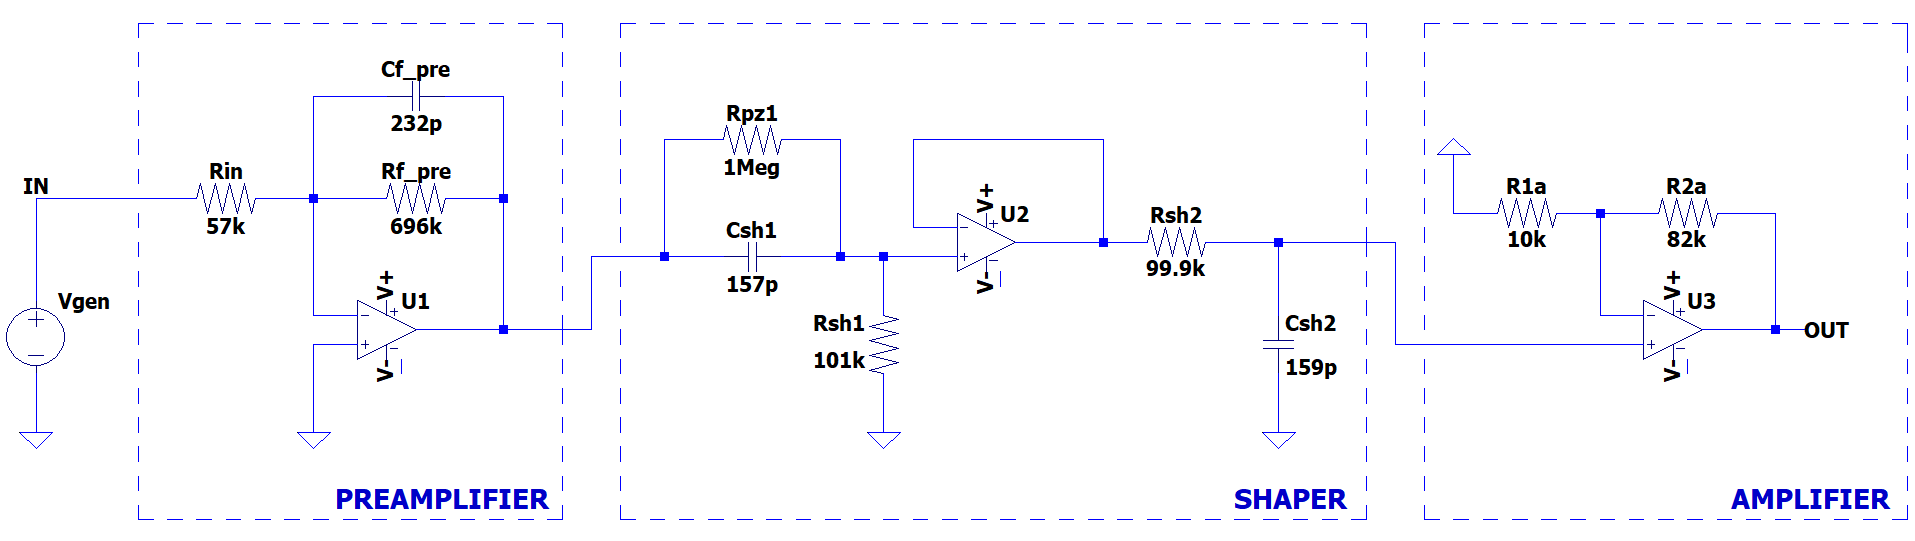
\includegraphics[width=\linewidth]{../Simulations/catena_circuito.png}
	\caption{\small Schema a costanti concentrate della catena elettronica suddivisa nei tre moduli di interesse.}
	\label{i:circuito}
\end{figure}

%-------------------------------------------------------------------------------------------------------------------------------------------
%	PREAMPLIFICATORE
%-------------------------------------------------------------------------------------------------------------------------------------------

\section{Preamplificatore}\label{s:preamp} 

Il primo stadio della catena \textit{(preamplificatore)} si utilizza per migliorare il rapporto segnale/rumore, in modo
da trasferire un segnale più pulito all'elettronica di acquisizione. Si assembla in laboratorio un preamplificatore
\textit{charge sensitive}: come si può osservare in \autoref{i:circuito} il modulo consiste di un circuito integratore
e la tensione in uscita è quindi direttamente proporzionale alla carica in ingresso. Lo scopo di questa sezione,
dedicata al preamplificatore, è di studiare il segnale in uscita verificandone l'integrazione e la linearità rispetto
alla carica in ingresso, oltre alla risposta in frequenza del filtro passa basso ricercandone la frequenza di taglio.

%-------------------------------------------------------------------------------------------------------------------------------------------
%	CONFIGURAZIONE SPERIMENTALE
%-------------------------------------------------------------------------------------------------------------------------------------------

\subsection{Configurazione Sperimentale}\label{s:preamp_config}

Si comincia utilizzando il generatore per simulare i segnali del rivelatore, impostando sul CH1 un impulso quadrato di
frequenza $f_{\text{gen}} = 1 \,\si{k\Hz}$, tensione di riferimento $V_{\text{high}} = 0 \,\si{\volt}$, ampiezza
\textit{negativa} $V_{\text{low}} = -1 \,\si{\volt}$ e durata $T = 5 \,\si{\us}$ (cioè il tempo di raccolta del
segnale). Viene successivamente assemblato 

\begin{wraptable}{L}{0.5\textwidth}
	\small
	\centering
	\begin{tabular}{x{1.8cm} x{2.5cm} x{2cm} } \toprule[0.5px]\toprule[0.1px]	
		\multicolumn{3}{c}{Misure Dirette - Preamplificatore}\tn
		\midrule[0.1px]
		Resistenza & Valore & F.S. \tn
		\addlinespace
		$R_{\text{in}}$ & $56.56 \pm 0.02\,\si{k\ohm}$ & $100\,\si{k\ohm}$ \tn
		$R_{\text{f}}$ & $696.1 \pm 0.3\,\si{k\ohm}$ & $1000\,\si{k\ohm}$ \tn
		$C_{\text{f}}$ & $0.232 \pm 0.009\,\si{n\farad}$ & $1\,\si{n\farad}$ \tn
		\bottomrule[0.5px]		
	\end{tabular}
	\caption{\footnotesize Misure dirette delle componenti circuitali.}
	\label{t:direct_measures}
\end{wraptable}	

\noindent sulla breadboard il primo modulo in \autoref{i:circuito} utilizzando le componenti circuitali riportate in
\autoref{t:direct_measures}, misurate con il multimetro Metrix. Si utilizza poi un generatore di tensione continua con
$V_{\text{cc}}=+15\,\si{\volt}$ e $V_{\text{ee}}=-15\,\si{\volt}$ per alimentare l'operazionale. Si assume, inoltre, che
esso abbia un comportamento ideale, ovvero che il polo positivo ed il polo negativo si trovino allo stesso potenziale
(\textit{virtual short}). Il segnale in ingresso $V_{\text{in}}$ viene prelevato nel punto \textit{IN} evidenziato nello
schema mentre il segnale in uscita $V^{\text{pre}}_{\text{out}}$ dal preamplificatore viene prelevato al termine del
primo modulo, entrambi utilizzando sonde 10X. Concentrando l'attezione sul modulo di ingresso (generatore reale e
cablaggio), il sistema è un filtro passa basso con frequenza di taglio $f_{\text{t}}^{\text{in}}\approx 32 \,\si{\MHz}$
che risulta essere molto maggiore delle frequenze in gioco: risulta allora corretto assumere il modulo in ingresso del
tutto equivalente ad un generatore ideale, come rappresentato in \autoref{i:circuito}. Trattando ora il preamplificatore,
la funzione di trasferimento del circuito risulta essere 
\begin{align}
	H(s) &= - \frac{ 1 }{ R_{\text{in}}\,C_{\text{f}} } \,\, \frac{1}{ s + \frac{ 1 }{ \tau_{\text{f}} } } & 
	&\text{con  } \,\, \tau_{\text{f}} = R_{\text{f}}\,C_{\text{f}} \equiv \tau^{\text{pre}}
\end{align}
\noindent Ricavando allora la risposta ad un segnale a gradino nell'approssimazione $T\ll\tau^{\text{pre}}$ si trova una
crescita lineare direttamente proporzionale alla corrente in ingresso al preamplificatore per $0 < t < T$ e una
decrescita smorzata esponenzialmente per $t \gg T$:
\begin{align}
	V^{\text{pre}}_{\text{out}}(t) &= 
	\begin{cases} 
		-\frac{ Q_{\text{in}} (t) }{ C_{\text{f}} } & 0 < t < T \\
		-\frac{ Q_{\text{c}} }{ C_{\text{f}} } \, e^{ -\frac{ t }{ \tau^{\text{pre}} } } & t \gg T \\
	\end{cases}
	& 
	&\text{con} \,\,\, 
	\begin{cases} 
		Q_{\text{in}} (t) = I_{\text{in}}\,t = \frac{ V_{\text{in}} }{ R_{\text{in}} }\,t \\
		Q_{\text{c}} = I_{\text{in}}\,T = \frac{ V_{\text{in}} }{ R_{\text{in}} }\,T \\
	\end{cases}
\end{align}	
\noindent dove, appunto, $Q_{\text{in}} (t)$ corrisponde alla carica raccolta al tempo $t$ dal preamplificatore mentre
$Q_{\text{c}}$ rappresenta la carica \textit{totale} accumulata nel preamplificatore. Ci si aspetta allora che il
segnale in uscita $V^{\text{pre}}_{\text{out}}$ visualizzato sull'oscilloscopio presenti una salita lineare, un valore
di tensione massimo corrispondente a $V_{\text{max}}^{\text{pre}} = 0.388 \pm 0.017 \,\si{\volt}$ (misurando l'ampiezza
del segnale in ingresso $V_{\text{in}} = 1.02 \pm 0.02 \,\si{\volt}$), e successivamente una decrescita esponenziale di
tempo caratteristico $\tau^{\text{pre}} = 0.161 \pm 0.006 \,\si{n\farad}$.


















\cleardoublepage
\subsection{Acquisizione Misure}\label{s:preamp_misure}
\subsection{Dati e Analisi}\label{s:preamp_analisi}
























%\section{Shaper}\label{s:shaper}
%
%\subsection{Configurazione Sperimentale}\label{s:shaper_config}
%\subsection{Acquisizione Misure}\label{s:shaper_misure}
%\subsection{Dati e Analisi}\label{s:shaper_analisi}
%
%\section{Catena Elettronica Completa}\label{s:catena}
%
%\subsection{Configurazione Sperimentale}\label{s:catena_config}
%\subsection{Acquisizione Misure}\label{s:catena_misure}
%\subsection{Dati e Analisi}\label{s:catena_analisi}
%
%\section{Conclusioni}














%----------------------------------------------------END OF FILE----------------------------------------------------------------------------
\end{document}